\documentclass[11pt]{article}
\title{\textbf{Meccano octagons}}
\author{https://github.com/heptagons/meccano/octa}
\date{}

\usepackage{amsmath}
\usepackage{listings}
\usepackage{xcolor}
\definecolor{gray}{RGB}{245,245,245}
\usepackage{float}
\usepackage{multicol}

\lstset{
	backgroundcolor=\color{gray},
	frame=single,
	numbers=left,
	stepnumber=1,
	tabsize=2,
	basicstyle=\ttfamily\small,
	breaklines=true
}

\usepackage[margin=0.75in]{geometry}

\usepackage{tikz}
\usetikzlibrary{math}
\usepackage{graphicx}
\usepackage{hyperref}
\usepackage{multicol}

\begin{document}

\maketitle
\begin{abstract}
We construct meccano\footnote{
\href{https://webspace.science.uu.nl/~hooft101/lectures/meccano.pdf}{Meccano mathematics by `t Hooft }
}
regular octagons using eight equal strips to build the a perimeter and attaching \textbf{internal diagonals} to make the polygon regular and rigid. The attached diagonals form angles of $135^\circ{}$ to fix consecutive sides. We prepare a three variables formula $z = f(x,y)$ and catalog solutions
when the variables are integers.
\end{abstract}

\newcommand{\rod}[4][000000] % [color]{n}{sep}{prop}
{
 \definecolor{main}{HTML}{#1}
 \draw[main] (0,{{2*#4}})
   -- ++({#2*#3},0) arc(+90:-90:{2*#4})
   -- ++({-#2*#3},0) arc(270:90:{2*#4});
 \foreach \x in {0,1,...,#2}
  \draw[main] (\x*#3,0) circle (#4);
}

\begin{figure}[H] %don't float
\centering
\scalebox{0.9}{
 \begin{tikzpicture}
 \def\p{3pt}
 \begin{scope}[rotate=-90]
  \draw[dash dot] (0,0) -- (6,6) node[midway,above right,black]{$\sqrt{2}z$};
  \begin{scope}[rotate=64.5]
   \draw (0,0) -- (9,0) node[midway,above right,black]{x};
   \rod[FF3300]{9}{1}{\p} % ADn
   \end{scope}
   \rod{6}{1}{\p} % AB
   \path (0,0) ++(222:5*\p) node{A};
   \begin{scope}[shift={(6,0)},rotate=90]
    \rod[009900]{6}{1}{\p} % BC
    \path (0,0) ++(222:5*\p) node{B};
    \begin{scope}[shift={(6,0)},rotate=45]
     \draw (0,0) -- (3,0) node[midway,above left,black]{y};
     \rod[009900]{6}{1}{\p} % CE
     \path (0,0) ++(222:5*\p) node{C};
     \path (1,0) ++(-90:5*\p) node{$D_1$};
     \path (2,0) ++(-90:5*\p) node{$D_2$};
     \path (3,0) ++(-90:5*\p) node{$D_n$};
     \path (4,0) ++(-90:5*\p) node{...};
     \path (6,0) ++(-75:5*\p) node{E};
    \end{scope}
   \end{scope}
   \begin{scope}[shift={(2,0)},rotate=37] %FG
    \rod[0033FF]{5}{1}{\p}
    \path (0,0) ++(75:5*\p) node{F};
    \path (5,0) ++(115:5*\p) node{G};
   \end{scope}
  \end{scope}
 \end{tikzpicture}
}
\caption{Construction of a $135^\circ{}$ angle with meccano strips.}
\label{fig:plan}
\end{figure}

\section{Meccano regular octagons}

We build meccano regular octagons forming rigid strips with internal angles of $135^\circ{}$. 
Figure \ref{fig:plan} show the internal diagonals construction. First, we build two
triangles with adjacent angles adding $135^\circ{}$. Consider triangle $ABC$ with
$\angle{BCA} = 45^\circ{}$ and triangle $ACD_n$ with $\angle{ACD_n} = 90^\circ{}$,
so $\angle{BCE} = 135^\circ{}$. Lets define:
\begin{align*}
x &= \overline{AD_n}\\
y &= \overline{CD_n}\\
z &= \overline{AB} = \overline{BC} = \overline{CE}
\end{align*}

The internal diagonal we are looking for is the integer $x$ (shown in red) and the two
adjacent octagon sides are $z = \overline{BC} = \overline{CE}$ (shown in green).
The two angles common hyphotenuse is shown as a dashed line with a length of $\overline{AC} = \sqrt{2}z$ so:
\begin{align*}
(\sqrt{2}z)^2 &= x^2 - y^2\\
         2z^2 &= x^2 - y^2\\
            z &= \sqrt{\frac{x^2 - y^2}{2}}
\end{align*}

We run a program using the above formula to iterate over integers pair $x > y$ and 
expecting to find $z$ as an integer too.

\subsection{Program}
Next golang listing program finds valid octagons diagonals $a$ and sides $\max(b,c)$.
First we iterate diagonals from 1 to a given maximum (line 2).
Then we iterate over integer $b$ from $1$ to $a$ (line 3).
We calculate $2c^2$ and check if its even (lines 4, 5) and the we check
if $c$ is an integer (line 8). To prevent repetitions by scaling we check
the greatest common divisor to be 1 (line 9) and print a valid result 
where the octagon size is the maximum value of $b$ or $c$. (line 11).
\begin{lstlisting}
func Angles135(max int) {
	for x := 1; x < max; x++ {
		for y := 1; y < x; y++ {
			if zz := x*x - y*y; zz % 2 == 0 {
				f := math.Sqrt(float64(zz / 2))
				if z := int(f); f == float64(z) {
					if meccano.Gcd(z, meccano.Gcd(x, y)) == 1 {
						a := int(math.Max(float64(y), f))
						fmt.Printf("a=%3d x=%3d y=%3d z=%3d\n", a, x, y, z)
					}
				}
			}
		}
	}
}
\end{lstlisting}

\subsection{Results}
First results for $x < 200$ are shown in the next listing.
The octagon size is $a = max(y,z)$.
\setlength{\columnsep}{100pt}
\begin{multicols}{2}
\begin{lstlisting}
a=  2 x=  3 y=  1 z=  2
a=  7 x=  9 y=  7 z=  4
a=  7 x= 11 y=  7 z=  6
a= 12 x= 17 y=  1 z= 12
a= 17 x= 19 y= 17 z=  6
a= 23 x= 27 y= 23 z= 10
a= 20 x= 33 y= 17 z= 20
a= 31 x= 33 y= 31 z=  8
a= 24 x= 41 y= 23 z= 24
a= 30 x= 43 y=  7 z= 30
a= 47 x= 51 y= 47 z= 14
a= 49 x= 51 y= 49 z= 10
a= 40 x= 57 y=  7 z= 40
a= 41 x= 57 y= 41 z= 28
a= 41 x= 59 y= 41 z= 30
a= 42 x= 67 y= 31 z= 42
a= 71 x= 73 y= 71 z= 12
a= 56 x= 81 y= 17 z= 56
a= 79 x= 83 y= 79 z= 18
a= 73 x= 89 y= 73 z= 36
a= 60 x= 97 y= 47 z= 60
a= 70 x= 99 y=  1 z= 70
a= 97 x= 99 y= 97 z= 14
a= 89 x=107 y= 89 z= 42
a= 72 x=113 y= 49 z= 72
a= 84 x=121 y= 23 z= 84
a= 73 x=123 y= 73 z= 70
a=119 x=123 y=119 z= 22
a=113 x=129 y=113 z= 44
a=127 x=129 y=127 z= 16
a= 90 x=131 y= 31 z= 90
a=119 x=137 y=119 z= 48
a=103 x=139 y=103 z= 66
a= 89 x=153 y= 89 z= 88
a=103 x=153 y=103 z= 80
a=161 x=163 y=161 z= 18
a=110 x=171 y= 71 z=110
a=167 x=171 y=167 z= 26
a=112 x=177 y= 79 z=112
a=161 x=177 y=161 z= 52
a=126 x=179 y= 17 z=126
a=137 x=187 y=137 z= 90
a=151 x=187 y=151 z= 78
a=132 x=193 y= 49 z=132
\end{lstlisting}
\end{multicols}

\newcommand{\fixer}[6] %{f}{p}{s}{d}{angle}{extra}
{
 \begin{scope}[shift={(#1*#6,0)}]
  \begin{scope}[rotate=90]
   \rod[000000]{#3}{#1}{#2}
   \begin{scope}[shift={(4*#1,0)},rotate=-143]
    \rod[0033FF]{5}{#1}{#2}
   \end{scope} 
   \begin{scope}[shift={(#1*#3,0)},rotate=-135+#5]
    \rod[FF3300]{#4}{#1}{#2}
   \end{scope} 
  \end{scope}
 \end{scope}
}

\newcommand{\octagon}[6] %{f}{p}{s}{d}{angle}{extra}
{
 \begin{tikzpicture}
  \pgfmathsetmacro{\s}{#3+#6}
  \begin{scope}
   \rod[009900]{\s}{#1}{#2} \path (0,0) ++(240:5*#2) node{A};
   \fixer{#1}{#2}{#3}{#4}{#5}{#6}
   \begin{scope}[shift={(\s*#1,0)},rotate=45]
    \rod[009900]{\s}{#1}{#2} \path (0,0) ++(240:5*#2) node{B};
    \fixer{#1}{#2}{#3}{#4}{#5}{#6}
    \begin{scope}[shift={(\s*#1,0)},rotate=45]
     \rod[009900]{\s}{#1}{#2} \path (0,0) ++(240:5*#2) node{C};
     \fixer{#1}{#2}{#3}{#4}{#5}{#6}
     \begin{scope}[shift={(\s*#1,0)},rotate=45]
      \rod[009900]{\s}{#1}{#2} \path (0,0) ++(240:5*#2) node{D};
      \fixer{#1}{#2}{#3}{#4}{#5}{#6}
      \begin{scope}[shift={(\s*#1,0)},rotate=45]
       \rod[009900]{\s}{#1}{#2} \path (0,0) ++(240:5*#2) node{E};
       \fixer{#1}{#2}{#3}{#4}{#5}{#6}
       \begin{scope}[shift={(\s*#1,0)},rotate=45]
        \rod[009900]{\s}{#1}{#2} \path (0,0) ++(240:5*#2) node{F};
        \begin{scope}[shift={(\s*#1,0)},rotate=45]
         \rod[009900]{\s}{#1}{#2} \path (0,0) ++(240:5*#2) node{G};
         \begin{scope}[shift={(\s*#1,0)},rotate=45]
          \rod[009900]{\s}{#1}{#2} \path (0,0) ++(240:5*#2) node{H};
         \end{scope}
        \end{scope}
       \end{scope}
      \end{scope}
     \end{scope}
    \end{scope}
   \end{scope}
  \end{scope}
 \end{tikzpicture}
}

\begin{figure}
\centering
\scalebox{0.5}{
 \octagon{2}{3pt}{4}{6}{19.5}{0}
}
\caption{The smallest octagon with diagonals $x=6$ and sides $z=4$.
In order to prevent bolts collisions we need to use strips with holes
well separated. Four $135^\circ{}$ units are needed to fix six consecutive rigid sides. This complex figure is simplified in next figure.}
\label{fig:smallest}
\end{figure}

\begin{figure}
\centering
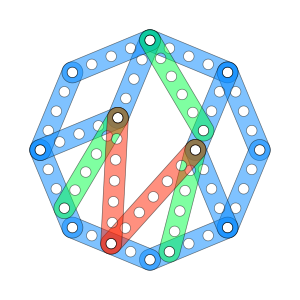
\includegraphics[]{figs/octagon-4}
\caption{The smallest octagon again with diagonals $x=6$ and sides $z=4$
but with fewer extra strips.
This construction is of the size of fig \ref{fig:smallest} but we put only
two adjacent $x$ red bars face to face and complete the rest with two
$z=4$ in blue and one more pythagorean green strip of size $5$.
}
\label{fig:smallest-simpler}
\end{figure}

\begin{figure}
\centering
\scalebox{0.5}{
 \octagon{1.4}{3pt}{4}{6}{19.5}{1}
}
\caption{Octagon with diagonals $x=6$ and sides $z+1=5$.}
\label{fig:second}
\end{figure}

\begin{figure}
\centering
\scalebox{1}{
 \octagon{0.5}{3pt}{4}{6}{19.5}{2}
}
\caption{Octagon with diagonals $x=6$ and sides $z+2=6$.}
\label{fig:third}
\end{figure}

\begin{figure}
\centering
\scalebox{1}{
 \octagon{0.5}{3pt}{4}{6}{19.5}{3}
}
\caption{Octagon with diagonals $x=6$ and sides $z+3=7$.}
\label{fig:fourth}
\end{figure}

\subsection{Examples with diagonal $x=6$}

We can't use the first result:
\begin{align*} 
a=2, x=3, y=1, z=2
\end{align*}
because the octagon size is to small, is only $z=2$.
At least the octagon size should be $4$ because the smallest right angle 
can be made with the pythagorean triplet $3$, $4$, $5$. To make rigid the angle of $90^\circ{}$ of triangle $ABC$ in figure \ref{fig:plan} we need a rod of size $5$ at least, as shown the points $F$ and $G$.
Multiplying the first result by $2$ we get:
\begin{align*}
a=4, x=6, y=2, z=4
\end{align*}
and this will be the smallest octagon since $z=4$ can hold a $3-4-5$ triplet.
Figure \ref{fig:smallest} is the smallest octagon; we need to scale the bars in order
the bolts don't collapse with others, the complexity of bars can be simplified 
symmetrically as is show in figure \ref{fig:smallest-simpler}.
In figure \ref{fig:second} we increase the side from $4$ to $5$ but keeping the same diagonal of $6$. In figure \ref{fig:third} we increase the side to $6$ and in figure
\ref{fig:fourth} the side is increased to $7$.


\subsection{Examples with diagonal $x=9$}

\begin{figure}
\centering
\scalebox{0.5}{
 \octagon{0.75}{3pt}{4}{9}{51}{3}
}
\caption{Octagon with diagonal $x=9$ and side $y=7$.}
\label{fig:9-7}
\end{figure}

\begin{figure}
\centering
\scalebox{0.5}{
 \octagon{0.5}{3pt}{4}{9}{51}{4}
}
\caption{Octagon with diagonal $x=9$ and side $y+1=8$.}
\label{fig:9-8}
\end{figure}


\begin{figure}
\centering
\scalebox{0.5}{
 \octagon{0.5}{3pt}{4}{9}{51}{5}
}
\caption{Octagon with diagonal $x=9$ and side $y+2=9$.}
\label{fig:9-9}
\end{figure}

\begin{figure}
\centering
\scalebox{0.7}{
 \octagon{0.5}{3pt}{4}{9}{51}{6}
}
\caption{Octagon with diagonal $x=9$ and side $y+3=10$.}
\label{fig:9-10}
\end{figure}

\begin{figure}
\centering
\scalebox{0.7}{
 \octagon{0.5}{3pt}{4}{9}{51}{7}
}
\caption{Octagon with diagonal $x=9$ and side $y+4=11$.}
\label{fig:9-11}
\end{figure}

With the second result:
\begin{align*}
a=7, x=9, y=7, z=4
\end{align*}
we can form a second group of octagons.
Figure \ref{fig:9-7} shows the smallest octagon with diagonals $9$
and sides $7$. Figures \ref{fig:9-8}, \ref{fig:9-9}, \ref{fig:9-10} and \ref{fig:9-11} show octagons with diagonals $9$ with sides of $8$, $9$, $10$ and $11$.

\subsection{Example with double diagonals $x=6$, $x=9$}

By comparing figures \ref{fig:fourth} and \ref{fig:9-10} both with sides=$y=7$ we can 
make use of two diagonals at the same time and omit the rod $FG$ of figure \ref{fig:plan} used until now to make the $90^\circ{}$ angle. Figure \ref{fig:diags2} show a
octagon angle with two diagonals. In other words, for two results or their scaling,
when both have the same $y$, we can use the two diagonals an omit the $5$ rod.

\begin{figure}[H] %don't float
\centering
\scalebox{0.8}{
 \begin{tikzpicture}
   \begin{scope}
    \def\f{1} \def\p{3pt}
    \rod[009900]{7}{\f}{\p}
    \path (0,0) ++(222:5*\p) node{A};
    \begin{scope}[shift={(7*\f,0)},rotate=45]
     \rod[009900]{7}{\f}{\p}
     \path (0,0) ++(222:5*\p) node{B};
     \path (7,0) ++(0:5*\p) node{C};
    \end{scope}
    \begin{scope}[shift={(3*\f,0)},rotate=90]   
     \rod{4}{\f}{\p}
     \path (0,0) ++(180:5*\p) node{D};
     \path (4,0) ++(60:5*\p) node{E};
     \begin{scope}[shift={(4*\f,0)},rotate=-135+19.5]
      \rod[FF3300]{6}{\f}{\p}
      \path (6,0) ++(0:5*\p) node{F};
     \end{scope}
     \begin{scope}[shift={(4*\f,0)},rotate=-135+51]
      \rod[FF3300]{9}{\f}{\p}
      \path (9,0) ++(-30:5*\p) node{G};
     \end{scope}
     
    \end{scope}
   \end{scope}
 \end{tikzpicture}
}
\caption{Octagon angle $ABC$ fixed with two diagonals.
The union of rods $\overline{BG}$, $\overline{EF}$ and $\overline{EG}$ is rigid.
Adding two rods $\overline{AB}$ and $\overline{DE}$ remains rigid.}
%\vspace{128in} %push to top
\label{fig:diags2}
\end{figure}


\end{document}